% TODO: Replace $A$, $B$ with $\alpha$, $\beta$?
% TDOO: Add several sentences about two scales.
% TODO: $A + B \cos 2x$ -> $A + \cos 2x$.
\documentclass[candidate, href, colorlinks]{disser}

\usepackage [T2A] {fontenc}
\usepackage [utf8] {inputenc}
\usepackage [english, main = russian] {babel}
\usepackage {tabularx}

\usepackage [intlimits] {amsmath}
\usepackage {amssymb}
\usepackage {amsfonts}
\usepackage [autostyle] {csquotes}
\usepackage {xcolor}
\usepackage {fancyhdr}
\usepackage {amsthm}
\usepackage {algorithm}
\usepackage {algorithmic}
\usepackage {mathrsfs}
\usepackage {physics}
\usepackage {caption}

\usepackage[a4paper, mag=1000, left=2.5cm, right=1cm, top=2cm, bottom=2cm, headsep=0.7cm, footskip=1cm] {geometry}

\usepackage[
	bibstyle=gost-numeric,
	backend=biber,
	language=auto,
	hyperref=auto,
	autolang=other,
	defernumbers=true,
	movenames=false,
	sorting=none,
	maxbibnames=99
] {biblatex}

\addbibresource{bibliography.bib}

\pagestyle{footcenter} % page number at bottom center

\renewcommand*{\thefootnote}{[\arabic{footnote}]}

\captionsetup[algorithm]{
  labelfont = bf,
  labelsep = period
}

\makeatletter
\renewcommand{\ALG@name}{Алгоритм}
\makeatother

\newtheorem{proposition}{Утверждение}

\begin{document}

% -------------------- TITLE -------------------- %
\begin{titlepage}
\thispagestyle{empty}
\enlargethispage{1cm}
\vspace*{-2cm}

\begin{center}
	Институт математики с вычислительным центром \\ УФИЦ РАН
\end{center}

\vskip1cm
	
\begin{flushright}
	\emph{На правах рукописи}
\end{flushright}
	
\vskip3cm

\begin{center}
	{\large Лебедев Михаил Евгеньевич}
	\vskip1cm
	{\Large\bfseries Стационарные состояния конденсата \\ Бозе--Эйнштейна в нелинейных решётках: \\ математическое и численное исследование \par}
	\vskip1.5cm
	{РЕЗЮМЕ ДИССЕРТАЦИИ \\ на соискание ученой степени кандидата наук \\ по прикладной математике}
\end{center}

\vskip2cm

\hspace{8cm}\begin{minipage}{0.4\linewidth}
	Научный руководитель \\
	д.~ф.-м.~н., проф. \\
	Алфимов Георгий Леонидович
\end{minipage}

\vfill

\begin{center}
	{Москва -- \the\year}
\end{center}

\normalfont\clearpage
\end{titlepage}
% -------------------- END -------------------- %

% ---------- GENERAL INFORMATION PAGE --------- %
%\addtocounter{page}{1}
%\thispagestyle{empty}
%\vspace*{-2cm}
%\noindent
%\begin{center}
%Работа выполнена в \emph{ИМВЦ УФИЦ РАН}.
%\end{center}
%\vskip1ex\noindent
%\begin{tabularx}{\linewidth}{@{}lX@{}}
%	\textbf{Научный руководитель:} & \textbf{Алфимов Георгий Леонидович}\\
%	& доктор физико-математических наук \\[6pt]
%	
%	\textbf{Официальные оппоненты:} & \textbf{\textcolor{red}{фамилия имя отчество}}\\
%	& \textcolor{red}{ученая степень, ученое звание} \\[6pt]
%	& \textbf{\textcolor{red}{фамилия имя отчество}} \\
%	& \textcolor{red}{ученая степень, ученое звание} \\[6pt]
%	
%	\textbf{Ведущая организация:} & Институт математики с вычислительным центром УФИЦ РАН
%\end{tabularx}
%
%\vskip5ex\noindent
%Защита состоится \datefield{} в \rule[0pt]{1cm}{0.5pt} часов
%на заседании диссертационного совета \emph{\textcolor{red}{шифр совета}} при \emph{\textcolor{red}{название организации, при которой создан совет}}, расположенном по адресу: \emph{\textcolor{red}{адрес}}.
%
%\vskip1ex\noindent
%С диссертацией можно ознакомиться в библиотеке \emph{\textcolor{red}{название организации}}, а также по ссылке \href{http://www.xyz.com}{\textcolor{red}{http://www.xyz.com}}.
%
%\vskip1ex\noindent
%Автореферат разослан \datefield{}
%
%\vskip2ex\noindent
%Отзывы и замечания по автореферату в двух экземплярах, заверенные
%печатью, просьба высылать по вышеуказанному адресу на имя ученого секретаря диссертационного совета.
%
%\vfill\noindent
%\begin{minipage}[b]{1\linewidth}
%	Ученый секретарь \\
%	диссертационного совета, \\
%	\emph{кандидат физико-математических наук}, \emph{доцент} \hfill \emph{Самбурский Л. М.}
%\end{minipage}
%
%\clearpage
% -------------------- END -------------------- %

\nsection{Общая характеристика работы}

\textbf{Введение.}
Начиная с 90-х годов прошлого века, нелинейное уравнение Шрёдингера (НУШ) с дополнительной пространственной неавтономностью продолжает оставаться объектом пристального изучения.
Интерес к этому классу уравнений во многом обусловлен экспериментальными успехами в исследовании конденсата Бозе--Эйнштейна (БЭК).
Явление конденсации вещества при сверхнизких температурах было предсказано в работах Бозе и Эйнштейна в 1924 году\footnote{A. Einstein, ``Quantentheorie des einatomigen idealen Gases'', Preussische Akademie der Wissenschaften, Berlin, 1924.}.
Экспериментально такое состояние вещества получено впервые в 1995 году независимо двумя группами исследователей\footnote{M. H. Anderson, J. R. Ensher, M. R. Matthews, C. E. Wieman, E. A. Cornell, ``Observation of Bose--Einstein Condensation in a Dilute Atomic Vapor'', Science, (New Series), Vol. 269, P. 198-201, 1995.}.
В 2001 году это открытие было удостоено Нобелевской Премии.

Возможность получение БЭК стимулировала экспериментальные и теоретические исследования по всему миру, открывшие целый ряд потенциальных практических приложений.
В частности, ожидается, что использование БЭК должно привести к появлению новых высокочастотных интерферометров\footnote{C. Gross, T. Zibold, E. Nicklas, J. Esteve, and M. K. Oberthaler, ``Nonlinear atom interferometer surpasses classical precision limit'', Nature, Vol. 464, P. 1165--1169, 2010.}.
Также БЭК может быть использован для построения квантовых компьютеров\footnote{D. Jaksch, P. Zoller, ``The cold atom Hubbard toolbox'', Annals of Physics, Vol. 315, P. 52--79, 2005.} и квантовых лазеров\footnote{W. Guerin, J.-F. Riou, J. P. Gaebler, V. Josse, P. Bouyer, and A. Aspect, ``Guided Quasicontinuous Atom Laser'', Phys. Rev. Lett., Vol. 97, P. 200402, 2006.}.

Динамика БЭК в приближении среднего поля описывается уравнением шредингеровского типа с пространственной неавтономностью.
\begin{equation}
	i \Psi_t + \Psi_{xx} - U(x) \Psi + P(x) |\Psi^2| \Psi = 0.
\label{eq:gpe}
\end{equation}
В контексте теории БЭК уравнение типа \eqref{eq:gpe} носит название {\it уравнения Гросса -- Питаевского}.
Здесь $\Psi(t, x)$ представляет обезразмеренную волновую функцию облака конденсата, которое предполагается вытянутым вдоль оси $x$.
Функция $U(x)$ описывает потенциал ловушки, удерживающей конденсат, а $P(x)$ соответствует нелинейному потенциалу, называемому также {\it псевдопотенциалом}.
Псевдопотенциал $P(x)$ описывает зависимость длины рассеяния частиц конденсата от пространственной координаты, которая может быть искусственно смоделирована различными экспериментальными техниками, например, использованием так называемого резонанса Фешбаха\footnote{C. Chin, R. Grimm, P. Julienne, and E. Tiesinga, ``Feshbach resonances in ultracold gases'', Rev. Mod. Phys. Vol. 82, P. 1225, 2010.}.
Интервалы с положительным значением псевдопотенциала $P(x) > 0$ соответствуют случаю межатомного притяжения, в то время как интервалы с отрицательным значением, $P(x) < 0$, ---  межатомному отталкиванию частиц конденсата.
Классическими модельными примерами потенциала $U(x)$ является гармонический потенциал $U(x) = Ax^2$ (магнитная ловушка), периодический потенциал $U(x) = A \cos 2x$ (оптическая ловушка), а также потенциальные ямы различных типов.

В качестве модельных примеров псевдопотенциала $P(x)$ используются различные функции, в том числе периодические.
В последнем случае говорят о воздействии на конденсат {\it нелинейной решётки}.
В экспериментах нелинейная решётка создается резонансным воздействием на конденсат дополнительного магнитного\footnote{S. Inouye, M. R. Andrews, J. Stenger, H.-J. Miesner, D. M. Stamper-Kurn \& W. Ketterle, ``Observation of Feshbach resonances in a Bose--Einstein condensate'', Nature, Vol. 392, P. 151-154, 1998.} или оптического\footnote{L. W. Clark, Li-Chung Ha, Chen-Yu Xu, and Cheng Chin, ``Quantum Dynamics with Spatiotemporal Control of Interactions in a Stable Bose--Einstein Condensate'', Phys. Rev. Lett., Vol. 115, P. 155301, 2015.} поля.
Присутствие нелинейной решётки открывает дополнительные возможности для стабилизации конденсата и для возбуждения в нём новых состояний.
Для моделирования нелинейной решётки в теоретических работах традиционно используется косинусный псевдопотенциал $P(x) = A + B \cos \Omega x$\footnote{\label{note:malomed} H. Sakaguchi,  B. A. Malomed, ``Matter-wave solitons in nonlinear optical lat­tices'', Phys. Rev. E, Vol. 72, P. 046610, 2005.}.

Стоит также отметить, что подобные задачи возникают и в других разделах физики, в частности в нелинейной оптике.
В оптических приложениях уравнение \eqref{eq:gpe} описывает распространение светового пучка в оптическом волокне, при этом периодическая пространственная модуляция нелинейности достигается добавлением в волокно резонантных примесей\footnote{J. Hukriede, D. Runde, and D. Kip, ``Fabrication and application of holographic Bragg gratings in lithium niobate channel waveguides'', J. Phys. D, Vol. 36, R1, 2003.}.

Для физических приложений важную роль играют решения уравнения \eqref{eq:gpe} специального вида --- так называемые {\it стационарные локализованные решения} ({\it стационарные локализованные моды}, СЛМ).
Они получаются в результате подстановки в соответствующее уравнение \eqref{eq:gpe} выражения
\begin{equation}
	\Psi(t, x) = u(x) e^{-i \omega t},
\label{eq:ansatz}
\end{equation}
где функция $u(x)$ удовлетворяет условию локализации:
\begin{equation}
	\lim \limits_{x \to \infty} u(x) = 0,
\label{eq:localization}
\end{equation}
а $\omega$ есть вещественный параметр, имеющий смысл химического потенциала конденсата.
Профиль стационарного локализованного решения $u(x)$ есть действительнозначная функция\footnote{G. L. Alfimov, V. V. Konotop, and M. Salerno, ``Matter solitons in Bose--Einstein condensates with optical lattices'', Europhys. Lett., Vol. 58, P. 7--13, 2002}, которая удовлетворяет уравнению
\begin{equation}
	u_{xx} + Q(x) u + P(x) u^3 = 0; \quad Q(x) = \omega - U(x).
\label{eq:stationary}
\end{equation}

Стоит отметить, что далеко не все локализованные решения уравнения \eqref{eq:stationary} одинаково интересны с физической точки зрения.
В частности, особо важным свойством является устойчивость локализованных решений.
Если СЛМ неустойчива, малые возмущения такого решения приводят к его разрушению при эволюции, описываемой уравнением \eqref{eq:gpe}.
Поэтому именно устойчивые локализованные решения особенно ценны для различных физических приложений, а сама проверка СЛМ на устойчивость является существенной частью их теоретического исследования.

\textbf{Постановка проблемы.}
Итак, при изучении динамики, описываемой уравнением \eqref{eq:gpe}, естественным образом возникают следующие вопросы:
\begin{enumerate}
	\item Возможно ли перечислить {\it полностью все} стационарные локализованные решения уравнения \eqref{eq:gpe}, одновременно существующие при заданных параметрах уравнения?
	\item Возможно ли эффективно выделить из этих решений те, которые являются устойчивыми?
\end{enumerate}

\textbf{Степень разработанности темы исследования.}
Стоит отметить, что в большинстве работ, посвящённых данной тематике вопрос о поиске / описании {\it всех} СЛМ не ставился.
Вместо него, как правило, рассматривался вопрос об отдельных классах СЛМ, соответствующих той или иной физической структуре, см. обзор\footnote{Y. V. Kartashov, B. A. Malomed, and L. Torner, ``Solitons in nonlinear lattices'', Rev. Mod. Phys. Vol. 83, P. 247, 2011.}.
В то же время, несмотря на некоторую <<амбициозность>> поставленных выше вопросов, сочетание строгих аналитических утверждений с численным счётом позволяет добиться существенных результатов в этом направлении. 
Отметим некоторые важные результаты.

Для уравнения \eqref{eq:stationary} c потенциалом $U(x)$, имеющего вид бесконечной потенциальной ямы, $U(x) = A x^2$, в случае отталкивающих взаимодействий, $P(x) \equiv -1$, был предложен метод <<доказательных вычислений>>, позволяющий гарантировать нахождение {\it всех} ограниченных решений при заданных значениях параметров задачи\footnote{\label{note:alfzez} G. L. Alfimov, D. A. Zezyulin, ``Nonlinear modes for the Gross--Pitaevskii equation --- a demonstrative computational approach'', Nonlinearity, Vol. 20, P. 2075--2092, 2007.}.
Разработанный метод впоследствии был обобщён на системы из нескольких связанных уравнений Гросса -- Питаевского, в которых соответствующие псевдопотенциалу коэффициенты также не зависят от пространственной координаты\footnote{G. L. Alfimov, I. V. Barashenkov, A. P. Fedotov, V. V. Smirnov, D. A. Zezyulin, ``Global search for localised modes in scalar and vector nonlinear Schr{\"o}dinger-type equations'', Physica D, Vol. 397, P. 39--53, 2019.}.

Для периодического потенциала $U(x)$ в случае отталкивающих взаимодействий частиц конденсата $P(x) \equiv -1$ предложены достаточные условия, опять же допускающие исчерпывающее описание {\it всех} ограниченных решений уравнения \eqref{eq:stationary}.
При этом показано, что выполнение этих условий позволяет установить взаимно-однозначное соответствие между ограниченными решениями и всевозможными бесконечными в обе стороны последовательностями символов из некоторого конечного алфавита\footnote{\label{note:alfavr} G. L. Alfimov, A. I. Avramenko, ``Coding of nonlinear states for the Gross--Pitaevskii equation with periodic potential'', Physica D, Vol. 254, P. 29--45, 2013.}.
Последовательности такого рода названы {\it кодами решений}, а сам процесс присвоения кодов -- {\it кодированием решений}.
Проверка достаточных условий проводилась авторами работы с помощью численного счёта.
Результаты предыдущей работы получили свое продолжение\footnote{G. L. Alfimov, P. P. Kizin, D. A. Zezyulin, ``Gap solitons for the repulsive Gross-Pitaevskii equation with periodic potential: Coding and method for computation'', Discrete and Continuous Dynamical Systems --- Series B, Vol. 22, P. 1207--1229, 2017.}, а именно: был разработан алгоритм, позволяющий по коду решения численно построить его профиль.

Стоит также отметить математические работы Ф. Занолина (F. Zanolin) и соавторов\footnote{Ch. Zanini, F. Zanolin, ``Complex Dynamics in One-Dimensional Nonlinear Schr\"odinger Equations with Stepwise Potential'', Complexity, Vol. 2018, Article ID 2101482, 2018.}\textsuperscript{,}\footnote{Ch. Zanini, F. Zanolin, ``An Example of Chaos for a Cubic Nonlinear Schr\"odinger Equation with Periodic Inhomogeneous Nonlinearity'', Advanced Nonlinear Studies, Vol. 12, No. 3, P. 481--499, 2012.}, в которых доказывается существование некоторых типов решений в близких задачах.
Эти решения также могут быть полностью описаны в терминах нелинейной динамики.
Авторы цитированных работ используют подход, отличающийся от представленного в данной работе и основывающийся на топологических аргументах.

\textbf{Актуальность темы исследования.}
Актуальной задачей является обобщение результатов приведенных выше работ на случай переменного псевдопотенциала $P(x) \neq \mathrm{const}$.
В частности, перспективным направлением исследования является обобщение аппарата кодирования решений на случай периодических потенциала и псевдопотенциала.
Детальная классификация решений уравнения \eqref{eq:gpe} открывает возможность экспериментального обнаружения новых, ранее неизвестных устойчивых СЛМ.

\textbf{Цели и задачи диссертационной работы.}
Основным объектом исследования данной диссертационной работы являются стационарные решения одномерного уравнения Гросса--Питаевского \eqref{eq:gpe} с {\it периодическим псевдопотенциалом}.
Цели и задачи работы можно сформулировать следующим образом:
\begin{enumerate}
	\item Сформулировать достаточные условия, дающие возможность обобщить метод кодировки СЛМ\textsuperscript{\ref{note:alfavr}} на случай периодического потенциала и периодического псевдопотенциала; указать способ проверки этих условий (аналитически или с помощью численного счета).
	\item Исследовать множество стационарных решений уравнения \eqref{eq:gpe} с периодическим псевдопотенциалом в случае принципиально нелинейных взаимодействий, когда линейным потенциалом можно пренебречь, $U(x) \equiv 0$.
	\item Для случая бесконечной потенциальной ямы, $U(x) = A x^2$, исследовать влияние периодического псевдопотенциала на структуру множества стационарных локализованных решений и их устойчивость.
\end{enumerate}

\textbf{Методология и методы исследования.}
Для исследования возможных типов СЛМ в работе используется так называемый <<метод исключения сингулярных решений>>\textsuperscript{\ref{note:alfavr}}.
Решение уравнения \eqref{eq:stationary} называется {\it сингулярным}, если оно уходит на бесконечность в конечной точке числовой прямой $x = x_0$:
\begin{equation}
	\lim \limits_{x \to x_0} u(x) = \infty.
\end{equation}
Очевидно, такие решения не могу описывать профиль волновой функции и должны быть исключены из рассмотрения.
При выполнении определенных условий <<большая часть>> решений уравнения \eqref{eq:stationary} представляет собой сингулярные решения.
Множество оставшихся решений, называемых {\it регулярными}, оказывается достаточно <<бедным>> и может быть полностью описано в терминах символической динамики.

Решение дифференциального уравнения \eqref{eq:stationary} производится с помощью метода Рунге--Кутта четвертого порядка точности.
Для построения локализованных решений уравнения \eqref{eq:stationary} в работе используется метод стрельбы.
Построенные решения проверяются на линейную устойчивость путём решения соответствующей задачи на собственные значения в пространстве Фурье (метод коллокаций Фурье\footnote{J. Yang, ``Nonlinear Waves in Integrable and Nonintegrable Systems'', Philadelphia: SIAM, 2010.}), а также посредством эволюционного моделирования динамики уравнения \eqref{eq:gpe} с помощью консервативной конечно-разностной схемы\footnote{V. Trofimov, N. Peskov Comparison of finite-difference schemes for the Gross-Pi­ taevskii equation // Mathematical Modelling and Analysis. — 2009. — Mar. — Vol. 14. — P. 109–126.}.
Все алгоритмы и численные методы реализованы в среде {\tt MATLAB} с использованием расширения {\tt MEX} для поддержки высокопроизводительных вычислений.

\textbf{Научная новизна.}
В диссертационной работе доказан ряд общих утверждение, указывающих, когда уравнение \eqref{eq:stationary} допускает существование сингулярных решений, а также, когда все его решения регулярны.
В частности, показано, что если псевдопотенциал принимает отрицательное значение хотя бы в одной точке $x_0$, $P(x_0) < 0$, то существуют два однопараметрических семейства решений, уходящих на бесконечность в этой точке, а также получены асимптотические формулы для этих семейств.

Дальнейшее развитие получает метод исключения сингулярных решений.
В работе предложены достаточные условия существования взаимно-однозначного соответствия между регулярными решениями уравнения \eqref{eq:stationary} и бесконечными последовательностями символов над некоторым алфавитом.
В отличии от ранее полученных результатов\textsuperscript{\ref{note:alfavr}}, предложенные достаточные условия могут быть эффективно проверены с помощью численного счета.
В диссертации приводится алгоритм их численной проверки, а также его теоретическое обоснование.

Для случая $U(x) \equiv 0$ и модельного периодического псевдопотенциала вида $P(x) = A + B \cos 2x$ исследовано множество стационарных локализованных решений.
Использование выше упомянутых техник позволило эффективно описать множество СЛМ и в конечном счёте обнаружить новое устойчивое решение, которое ранее не обсуждалось в литературе при рассмотрении задач, связанных с уравнением \eqref{eq:gpe}.
Найденное новое устойчивое решение получило название {\it дипольный солитон} \cite{LebedevAlfimovMalomed}.

Наконец, изучен вопрос о влиянии периодического псевдопотенциала вида $P(x) = A + B \cos \Omega x$ на множество СЛМ в случае бесконечной потенциальной ямы, $U(x) = A x^2$.
Показано, что по сравнению с хорошо изученным случаем $P(x) = \mathrm{const}$, множество стационарных локализованных решений оказывается значительно богаче, а именно, появляются существенно нелинейные решения, не существующие в малоамплитудном пределе.
Исследована зависимость устойчивости СЛМ от частоты псевдопотенциала $\Omega$.
Для псевдопотенциала с нулевым средним, $P(x) = B \cos \Omega x$, показано, что увеличение частоты $\Omega$ позволяет стабилизировать малоамплитудные решения, чьи аналоги в модели с $P(x) = \mathrm{const}$ оказываются неустойчивыми.

% \textbf{Теоретическая и практическая значимость.}
% Результаты, изложенные в диссертации, могут быть использованы при проведении экспериментов с конденсатом Бозе--Эйнштейна.

\textbf{Положения, выносимые на защиту:}
\begin{enumerate}
	\item Сформулированы и доказаны общие утверждения о наличии и отсутствии сингулярных решений уравнения \eqref{eq:stationary}.
		Показано, что в случае $P(x) > 0$ все решения уравнения \eqref{eq:stationary} регулярны.
		Если $P(x)$ принимает отрицательное значение хотя бы в одной точке $x_0$, $P(x_0) < 0$, то существуют два однопараметрических семейства решений, уходящих на бесконечность в точке $x = x_0$; построена асимптотика этих решений. 
		В том случае, когда $Q(x) < 0$ и $P(x) < 0$, показано, что все решения уравнения \eqref{eq:stationary} сингулярны.
	\item Сформулированы достаточные условия возможности кодирования регулярных решений уравнения \eqref{eq:stationary} и предложен эффективный алгоритм численной проверки этих условий.
	\item Для случая $U(x) \equiv 0$, $P(x) = A + \cos 2x$ исследовано множество СЛМ уравнения \eqref{eq:gpe} и обнаружено новое устойчивое локализованное решение --- {\it дипольный солитон}.
	\item В случае бесконечной потенциальной ямы вида $U(x) = A x^2$ показано, что присутствие периодического псевдопотенциала приводит к появлению новых классов СЛМ, не имеющих аналогов в моделях с $P(x) = \mathrm{const}$.
		Для псевдопотенциала с нулевым средним установлено, что частота псевдопотенциала существенным образом влияет на устойчивость СЛМ.
		Установлено, что увеличение частоты приводит к стабилизации малоамплитудных стационарных локализованных решений.
\end{enumerate}

\textbf{Степень достоверности и апробация результатов.}
Модель Гросса -- Питаевского является классической моделью физики сверхнизких температур и её достоверность не вызывает сомнений.
В данной диссертационной работе численно строятся локализованные стационарные решения указанной модели, а также численно исследуется устойчивость таких решений.
Построение решений производится при помощи стандартных численных методов с контролируемой точностью.
Исследование устойчивости построенных решений производится спектральным методом, который хорошо зарекомендовал себя для решения подобных задач.
Результаты исследования устойчивости проверяются численным решением эволюционной задачи при помощи конечно-разностной схемы.
Основные результаты диссертационной работы докладывались на различных научных семинарах и конференциях, в числе которых:
\begin{enumerate}
	\item <<Фундаментальная математика и ее приложения в естествознании>>, БашГУ, Уфа, сентябрь, 2015 г.
	\item <<Динамика, бифуркации и странные аттракторы>>, Нижегородский государственный университет, Нижний Новгород, июль, 2016 г.
	\item <<Комплексный анализ, математическая физика и нелинейные уравнения>>, Башкортостан, оз. Банное, март, 2018 г.
	\item ``Nonlinear Phenomena in Bose Condensates and Optical Systems'', Ташкент, Узбекистан, август, 2018 г.
	\item <<Комплексный анализ, математическая физика и нелинейные уравнения>>, Башкортостан, оз. Банное, март, 2019 г.
	\item <<Комплексный анализ, математическая физика и нелинейные уравнения>>, Башкортостан, оз. Банное, март, 2021 г.
\end{enumerate}

\textbf{Публикации.}
Материалы диссертации опубликованы в 9 печатных работах, из них 3 статьи в рецензируемых журналах \cite{AlfimovLebedev, LebedevAlfimovMalomed, AlfimovGegelLebedevMalomedZezyulin} и 6 тезисов докладов на различных конференциях \cite{Ufa2015, NizhniNovgorod2016, Bannoe2018, Tashkent2018, Bannoe2019, Bannoe2021}.
Также за время работы над диссертацией автором было опубликовано 2 статьи\footnote{M. E. Lebedev, D. A. Dolinina, K. B. Hong, {\it et al.}, ``Exciton-polariton Josephson junctions at finite temperatures'', Scientific Reports Vol. 7, P. 9515, 2017}\textsuperscript{,}\footnote{D. A. Zezyulin, M. E. Lebedev, G. L. Alfimov, and B. A. Malomed, ``Symmetry breaking in competing single-well linear-nonlinear potentials'', Phys. Rev. E, Vol. 98, P. 042209, 2018.} по смежным тематикам (результаты одной из этих работ также докладывались на конференции\footnote{D. A. Zezyulin, M. E. Lebedev, G. L. Alfimov, and B. A. Malomed, ``Symmetry breaking in competing single-well linear-nonlinear potentials'', Тезисы доклада на конференции <<Комплексный анализ, математическая физика и нелинейные уравнения>>, Башкортостан, оз. Банное, март, 2019.}).

\textbf{Личный вклад автора.}
Содержание диссертации и основные положения, выносимые на защиту, отражают персональный вклад автора в опубликованные работы.
Подготовка к публикации полученных результатов проводилась совместно с соавторами, причем вклад диссертанта был определяющим.
Все представленные в диссертации результаты получены лично автором с использованием разработанных методов и компьютерных программ.

\textbf{Структура и объем диссертации.}
Диссертация состоит из введения, четырёх глав, трёх приложений и библиографии.
Общий объем диссертации 130 страниц, из них 115 страниц текста, включая 35 рисунков, 4 таблицы и 1 схему алгоритма.
Библиография включает 61 наименование на 8 страницах.

\nsection{Содержание работы}

Во \textbf{введении (Introduction)} обоснована актуальность диссертационной работы, сформулирована цель и аргументирована научная новизна исследований, показана практическая значимость полученных результатов, представлены выносимые на защиту научные положения.

Вводятся основные понятия, относящиеся к объекту исследования.
{\it Стационарные локализованные решения} (или {\it стационарные локализованные моды}, СЛМ) определяются как решения уравнения \eqref{eq:gpe}, имеющие вид \eqref{eq:ansatz} и удовлетворяющие условию локализации \eqref{eq:localization}.
Решение $u(x)$ уравнения \eqref{eq:stationary} называется {\it сингулярным}, если для некоторой конечной точки $x_0$ выполняется $u(x) \to \infty$ при $x \to x_0$.
Точка $x_0$ называется точкой коллапса решений, а про само решение говорится, что оно {\it коллапсирует} в точке $x_0$.
Решение называется {\it регулярным}, если оно не коллапсирует ни в какой точке.

В \textbf{первой главе (Chapter I)} сформулированы и доказаны основные утверждения о сингулярных и регулярных решениях уравнения \eqref{eq:stationary}.

\begin{proposition}
\label{prop:absense-of-singular-solutions}
	Пусть для всех $x \in \mathbb{R}$, в уравнении \eqref{eq:stationary} функции $Q(x), \, P(x) \in C^1(\mathbb{R})$, причём
	\begin{enumerate}
		\item[(a)] $P(x) \ge P_0 > 0$, $|P'(x)| \le \widetilde{P}$;
		\item[(б)] $Q(x) \ge Q_0$, $|Q'(x)| \le \widetilde{Q}$.
	\end{enumerate}
	Тогда решение задачи Коши для уравнения \eqref{eq:stationary} с произвольными начальными условиями может быть продолжено на всю действительную ось $\mathbb{R}$.
\end{proposition}

Утверждение \ref{prop:absense-of-singular-solutions} устанавливает условия отсутствия сингулярных решений.
Одним из таких условий является положительность функции $P(x)$ на всей числовой прямой.
Если же функция $P(x)$ принимает отрицательное значение хотя бы в одной точке $x_0$, $P(x_0) < 0$, это порождает два семейства решений уравнения \eqref{eq:stationary}, коллапсирующих в этой точке.
Для формулировки следующего утверждения удобно положить $P(x_0) = -1$ (этого всегда можно добиться путём соответствующей перенормировки).

\begin{proposition}
\label{prop:singular-families}
	Пусть $\Omega$ --- некоторая окрестность точки $x_0$, а $Q(x) \in C^2(\Omega)$ и $P(x) \in C^4(\Omega)$.
	Тогда существуют два $C^1$-гладких однопараметрических семейства решений уравнения \eqref{eq:stationary}, коллапсирующих в точке $x = x_0$ (при приближении слева, $x \to x_0{-}0$) и связанных между собой симметрией $u \to -u$.
	Каждое из этих семейств может быть запараметризовано свободной переменной $C \in \mathbb{R}$, причём для этих семейств справедливы следующие асимптотические разложения:
	\begin{equation}
		\pm u(x) = \dfrac{\sqrt{2}}{\eta} + A_0 + A_1 \eta + A_2 \eta^2 + A_3 \eta^3 \ln |\eta| + C \eta^3+ A_4 \eta^4 \ln |\eta| + \dots.
	\label{eq:expansion}
	\end{equation}
	Здесь $\eta = x - x_0$, а коэффициенты $A_n$ выражаются через коэффициенты $Q_n$, $P_n$ разложения функций $Q(x)$, $P(x)$
	\begin{equation}
		Q(x) = Q_0 + Q_1 \eta + Q_2 \eta^2 \dots, \quad P(x) = -1 + P_1 \eta + P_2 \eta^2 + \dots.
	\end{equation}
\end{proposition}

Аналогичные однопараметрические семейства коллапсирующих решений существуют также и справа от точки $x = x_0$.
Наконец, в первой главе устанавливаются условия, при которых уравнение \eqref{eq:stationary} вообще не имеет регулярных решений, за исключением нулевого решения $u(x) \equiv 0$.

\begin{proposition}
\label{prop:all-solutions-are-singular}
 	Пусть при $x \in \mathbb{R}$ выполняются условия $P(x) \le P_0 < 0$, $Q(x) \le Q_0 < 0$.
 	Тогда все решения уравнения \eqref{eq:stationary} сингулярны, за исключением нулевого решения.
\end{proposition}

Одним из следствий полученных результатов является то, что в том случае, когда псевдопотенциал $P(x)$ является знакопеременной функцией, сингулярность является характерным свойством большого количества решений уравнения \eqref{eq:stationary}, что, в свою очередь, делает возможным применение метода исключения сингулярных решений\textsuperscript{\ref{note:alfavr}}.
Результаты первой главы опубликованы в работах \cite{AlfimovLebedev} и \cite{Ufa2015}.

Во \textbf{второй главе (Chapter II)} представлен аппарат кодирования стационарных состояний уравнения \eqref{eq:gpe} с $L$-периодическими функциями потенциала, $U(x + L) = U(x)$, и псевдопотенциала, $P(x + L) = P(x)$.
Оказывается, что множество регулярных решений уравнения \eqref{eq:stationary} при определенных условиях можно полностью описать исходя из структуры так называемых {\it кодировочных множеств}: $\mathscr{U}_L^+$, $\mathscr{U}_L^-$, $\mathscr{U}_L$.
Эти множества определяются на плоскости $(u, u')$ начальных условий уравнения \eqref{eq:stationary} следующим образом.
Множество $\mathscr{U}_L^+$ содержит в себе начальные условия для решений, ограниченных на промежутке $[0; L]$, а множество $\mathscr{U}_L^-$ --- начальные условия для решений, ограниченных на промежутке $[-L; 0]$.
Множество $\mathscr{U}_L$ есть пересечение двух предыдущих множеств, $\mathscr{U}_L = \mathscr{U}_L^+ \cap \mathscr{U}_L^-$.
Связь между точками этих множеств удобно описать с помощью {\it отображения Пуанкаре} $\mathcal{P}$, которое определено следующим образом: пусть $\vb{p} \in \mathscr{U}_L^+$, тогда $\mathcal{P} (\vb{p}) = \vb{q} = (u(L), u'(L))$, $\vb{q} \in \mathscr{U}_L^-$, где $u(x)$ --- решение задачи Коши для уравнения \eqref{eq:stationary} с начальными условиями $u(0) = u_0$, $u'(0) = u_0'$.
Последовательность точек $\{ \vb{p}_n \}$, связанных отображением Пуанкаре, $\mathcal{P}(\vb{p}_n) = \vb{p}_{n + 1}$, называется {\it орбитой}.

Ключевым моментом на пути к описанию множества регулярных решения является выполнение {\it двух гипотез} относительно действия отображения $\mathcal{P}$ на множестве $\mathscr{U}_L$.
\begin{itemize}
	\item[(I)] Множество $\mathscr{U}_L$ представляет из себя набор компонент связности $\mathscr{U}_L = \bigcup_{k \in S} D_k$, где каждая компонента $D_k$ есть криволинейный четырехугольник с монотонными границами, а также для любых $i, j$ множества $H_{ij} = \mathcal{P}(D_i) \cap D_j$ и $V_{ij} = \mathcal{P}^{-1}(D_j) \cap D_i$ непустые. 
	\item[(II)] Отображения $\mathcal{P}$, $\mathcal{P}^{-1}$ некоторым образом сохраняют свойства монотонности полос, названных в работе {\it h- и v-полосами}, соединяющих противоположные стороны $D_k$, причем ширина этих полос убывает под действием соответствующих отображений.
\end{itemize}
Поясним гипотезу~II.
Если она верна, тогда определенные выше множества $H_{ij}$ и $V_{ij}$ представляют из себя h- и v- полосы соответственно.
Из гипотезы~II следует, что множества $\mathcal{P}(H_{ij}) \cap D_k$ также являются h-полосами, при этом выполняется неравенство $d_{\mathrm{h}}(\mathcal{P}(H_{ij}) \cap D_k) < d_{\mathrm{h}}(H_{ij})$, где под $d_{\mathrm{h}}(\cdot)$ понимается ширина h-полосы, измеряемая вдоль вертикальной прямой.
Аналогично множества $\mathcal{P}^{-1}(V_{ij}) \cap D_k$ представляют из себя v-полосы, причём верным оказывается неравенство $d_{\mathrm{v}}(\mathcal{P}^{-1}(V_{ij}) \cap D_k) < d_{\mathrm{v}}(V_{ij})$, где $d_{\mathrm{v}}(\cdot)$ есть ширина v-полосы, измеряемся вдоль горизонтальной прямой.

В данной главе показано, что при выполнении гипотез I и II отображение $\mathcal{P}$ действует на множестве $\mathscr{U}_L$ по схеме подковы Смейла\footnote{S. Wiggins, ``Introduction to Applied Nonlinear Dynamical Systems and Chaos'', New York: Springer-Verlag, 2003.}, и существует взаимно-однозначное соответствие между {\it орбитами} регулярных решений уравнения \eqref{eq:stationary} и {\it множеством бесконечных последовательностей}, в которых каждый символ соответствует компоненте связности множества $\mathscr{U}_L$.
В этой части работы автор следует подходу, описанному в работах Л.~П.~Шильникова и В.~М.~Алексеева в 60-70-e годы прошлого века.
В основных статьях\footnote{Л. П. Шильников, <<Об одной задаче Пуанкаре-Биркгофа>>, Математический сборник, Т. 74, \textnumero 4, С. 378--397,  1967.}\textsuperscript{,}\footnote{В. М. Алексеев, <<Финальные движения в задаче трех тел и символическая динамика>>, Успехи математических наук, Т. 36, Вып. 4, С. 161, 1981.} подход, основанный на символической динамике, был успешно применен к описанию поведения траекторий вблизи гомоклинической орбиты, а также для задачи трёх тел.
В данной работе такой подход применяется к динамике отображений $\mathcal{P}$, $\mathcal{P}^{-1}$, действующих на множествах $\mathscr{U}_L^{\pm}$, что является новым приложением этой теории.

Проверка гипотез осуществляется численно.
При этом гипотеза I может быть легко проверена {\it методом сканирования плоскости начальных условий}.
Проверка же гипотезы II не столь проста и требует более обстоятельного подхода.
В данной главе сформулированы две теоремы ({\it теоремы об отображении h- и v-полос}), которые позволяют свести проверку гипотезы II к эффективной численной процедуре.
Данная процедура заключается в вычислении значений элементов матрицы Якоби, а также оценке некоторых констант в точках $\vb{p}$, принадлежащих специальным подмножествам множества $\mathscr{U}_L$.
Сам алгоритм проверки выглядит следующим образом.

\begin{algorithm}[H]
\caption{Проверка гипотезы II}
\label{algorithm:hypotheses-validation}
\begin{algorithmic}
	\STATE \textbf{Дано:} Гипотеза I верна для уравнения \eqref{eq:stationary}; $\mathscr{U}_L = \bigcup_{k \in S} D_k$.
	\STATE \textbf{Шаг (1)}. Задать расчётную сетку.
		Для всех $i, j \in S$ численно построить множества $H_{ij} = \mathcal{P}(D_i) \cap D_j$, и $V_{ij} = \mathcal{P}^{-1} (D_j) \cap D_i$ на заданной расчётной сетке.
	\STATE \textbf{Шаг (2)}. Проверка знаков элементов в матрицах Якоби $D \mathcal{P}_{\vb{p}}$, $D \mathcal{P}_{\vb{q}}^{-1}$ для отображений $\mathcal{P}$, $\mathcal{P}^{-1}$.
	\STATE
	\begin{enumerate}
		\setlength{\itemsep}{1pt}
		\setlength{\parskip}{0pt}
  		\setlength{\parsep}{0pt}
		\item[\textbf{(а)}] Для $\vb{p} \in V_{ij}$ вычислить матрицу 2$\cross$2 оператора $D \mathcal{P}_{\vb{p}} = (a_{mn})$ и проверить, что знаки её элементов $\forall \vb{p} \in V_{ij}$ соответствуют в точности одной из конфигураций, указанных в теореме об отображении h-полос.
		\item[\textbf{(б)}] Для $\vb{q} \in H_{ij}$ вычислить матрицу 2$\cross$2 оператора $D \mathcal{P}_{\vb{q}}^{-1} = (b_{mn})$ и проверить, что знаки её элементов $\forall \vb{q} \in H_{ij}$ соответствуют в точности одной из конфигураций, указанных в теореме об отображении v-полос.
	\end{enumerate}
	\STATE \textbf{Шаг (3)}. Оценка сжатия h- и v-полос.
	\STATE
	\begin{enumerate}
		\setlength{\itemsep}{1pt}
		\setlength{\parskip}{0pt}
  		\setlength{\parsep}{0pt}
		\item[\textbf{(а)}] Используя расчётную сетку, оценить значение $\mu_* = \min \limits_{\vb{p} \in V_{ij}} a_{11}(\vb{p})$; проверить, что $\mu_* > 1$.
		\item[\textbf{(б)}] Используя расчётную сетку, оценить значение $\nu_* = \min \limits_{\vb{q} \in H_{ij}} b_{22}(\vb{q})$; проверить, что $\nu_* > 1$.
	\end{enumerate}
\end{algorithmic}
\end{algorithm}

Работа алгоритма (см. рисунок~\ref{fig:hypotheses-validation}) проиллюстрирована на примере уравнения \eqref{eq:stationary} с $Q(x) \equiv -1$ и $P(x) = \eta(x)$, где $\eta(x)$ --- кусочно-постоянная периодическая функция с периодом $L = L_* + L_0$, определенная следующим образом:
\begin{equation}
	\eta(x) = \left\{
		\begin{array}{rl}
			-1, & x \in [0; L_*); \\
			+1, & x \in [L_*; L_* + L_0).
		\end{array}
	\right.
\label{eq:eta}
\end{equation}
Оказывается (доказано строгое утверждение), что множество $\mathscr{U}_L$ на плоскости начальных условий для такого уравнения неограниченно.
Тем не менее можно ограничиться рассмотрением некоторого ограниченного подмножества $\mathcal{D} \subset \mathscr{U}_L$.
Если гипотезы I и II верны для $\mathcal{D}$, тогда можно описать подмножество регулярных решений, чьи орбиты не выходят за пределы рассмотренного подмножества $\mathcal{D}$ на плоскости начальных условий.
На рисунке~\ref{fig:hypotheses-validation} показан пример множества $\mathcal{D}$, состоящего из трёх компонент связности.
Гипотезы I и II верны для $\mathcal{D}$, а значит существует подмножество регулярных решений, которое может быть кодировано тремя символами $\{-1, 0, +1\}$.
Результаты второй главы опубликованы в работах \cite{Bannoe2019} и \cite{Bannoe2021}.

\begin{figure}[h]
\centering
	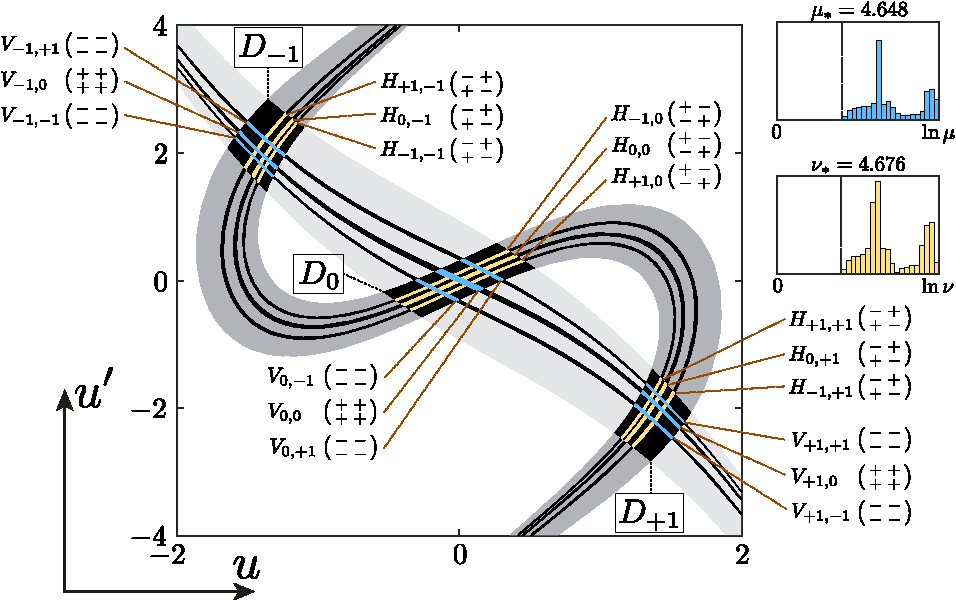
\includegraphics[scale = 1]{../pic/hypotheses for piecewise equation}
	\caption{
		Проверка гипотез для уравнения \eqref{eq:stationary} для случая $Q(x) \equiv -1$, $P(x) = \eta(x)$ с параметрами $(L_*, L_0) = (2, 1)$.
		Множество $\mathscr{U}_L^+$ (светло-серый), $\mathscr{U}_L^-$ (тёмно-серый), их пересечение $\mathcal{D} = \{ D_{-1}, D_0, D_{+1} \} \subset \mathscr{U}_L$ (чёрный); для множеств $V_{ij}$ (синий) и $H_{ij}$ (жёлтый) указаны знаки элементов соответствующих операторов.
	}
\label{fig:hypotheses-validation}
\end{figure}

В \textbf{третьей главе (Chapter III)} исследуется множество стационарных решения уравнения \eqref{eq:gpe}, в котором потенциал ловушки отсутствует, $U(x) \equiv 0$, а псевдопотенциал имеет вид косинуса, $P(x) = A + \cos 2x$.
Такая задача ранее рассматривалась в литературе\textsuperscript{\ref{note:malomed}}.
Было установлено, что она допускает стационарное локализованное решение колоколообразной формы, называемое {\it фундаментальный солитон}, которое является устойчивым при определенных параметрах уравнения.

В данной главе к такому уравнению применяется подход, основанный на методике кодирования решений.
Структура кодировочных множеств приведена на рисунке~\ref{fig:island-set}.
Оказывается, что множества $\mathscr{U}_{\pi}^{\pm}$ ($L = \pi$) представляют из себя бесконечные спирали, которые образуют неограниченное пересечение $\mathscr{U}_{\pi}$, состоящее из бесконечного количества компонент связности.

\begin{figure}[h]
\centering
	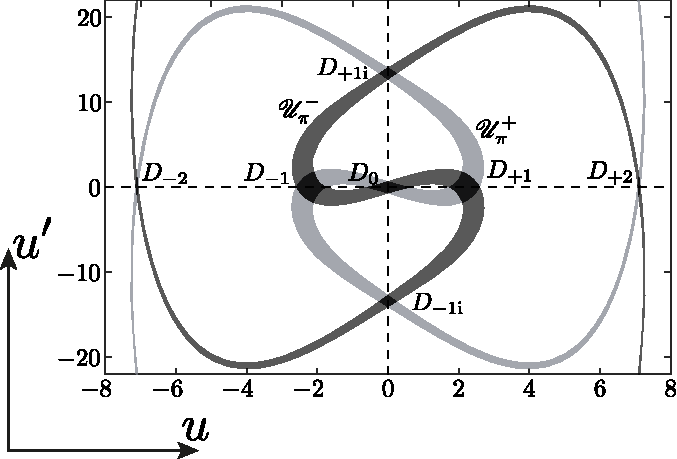
\includegraphics[scale = 1]{../pic/island set to check hypotheses for cosine equation}
	\caption{
		Множество $\mathcal{D} \subset \mathscr{U}_{\pi}$, состоящее из семи компонент связности $\{ D_{-2}, D_{-1\mathrm{i}}, D_{-1}, D_0, D_{+1}, D_{+1\mathrm{i}}, D_{+2} \}$ (чёрный), сформированное пересечением множеств $\mathscr{U}_{\pi}^{\pm}$ для уравнения \eqref{eq:stationary}; $Q(x) = -1.5$, $P(x) = \cos 2x$.
	}
\label{fig:island-set}
\end{figure}

Проверка гипотез I и II осуществляется для подмножества $\mathcal{D} \subset \mathscr{U}_{\pi}$, состоящего из семи центральных компонент связности.
Численная процедура проверки гипотез позволила заключить, что обе гипотезы верны.
Следовательно, существует взаимно-однозначное соответствие между решениями уравнения \eqref{eq:stationary} и кодами, построенными исходя из структуры кодировочного множества.
Наличие такого соответствия показывает, что множество стационарных локализованных решения рассматриваемого уравнения чрезвычайно богато.
На рисунке~\ref{fig:solutions} представлены различные решения и соответствующие им символьные коды.

Анализ линейно устойчивости спектральным методом показал, что большинство решений являются неустойчивыми, однако в задаче существует некоторое количество устойчивых решений, часть из которых ранее не была известна.
Одним из таких новых устойчивых решений является так называемый {\it дипольный солитон}, профиль которого изображен на рисунке~\ref{fig:solutions}~(e).
Результаты третьей главы опубликованы в работах \cite{LebedevAlfimovMalomed}, \cite{NizhniNovgorod2016} и \cite{Tashkent2018}.

\begin{figure}[h!]
\centering
	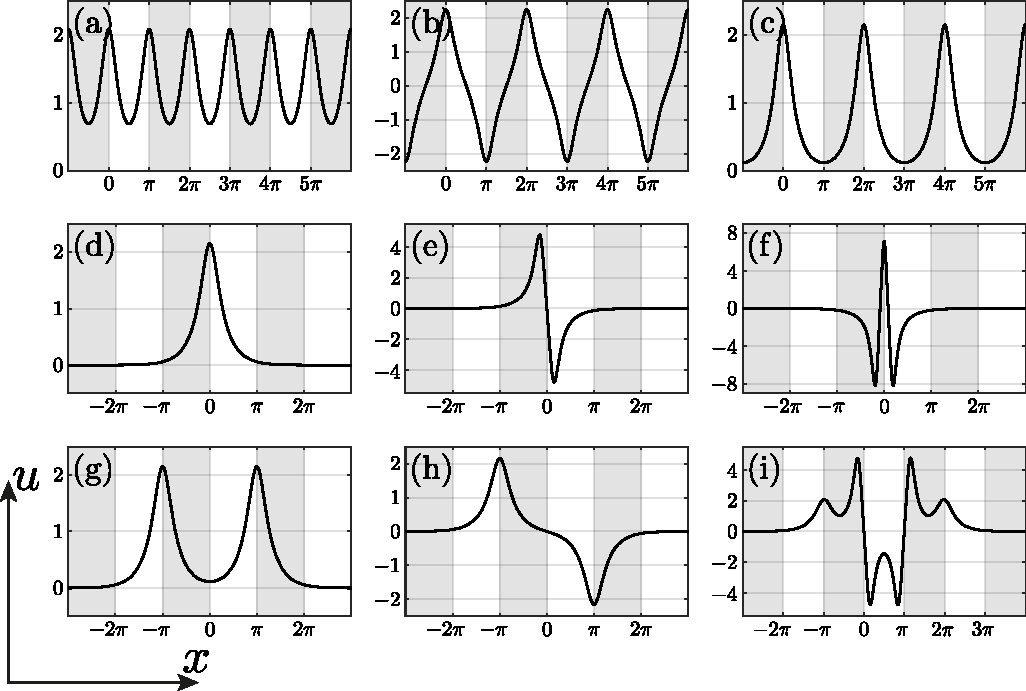
\includegraphics[scale = 1]{../pic/solutions for cosine equation}
	\caption{
		Различные решения уравнения \eqref{eq:stationary} для $Q(x) = -1.5$, $P(x) = \cos 2x$.
		Каждому решению соответствует символьный код, который однозначно идентифицирует решение.
		Периодические решения: (a) $\pi$-перидическое решение $\{ \dots, +1, +1, +1, \dots \}$; (b) $2 \pi$-периодическое решение $\{ \dots, +1, -1, +1, -1, \dots \}$; (c) $2 \pi$-периодическое решение $\{ \dots, +1, 0, +1, 0, \dots \}$.
		Локализованные решения: (d) фундаментальный солитон $\{ \dots, 0, +1, 0, \dots \}$; (e) дипольный солитон $\{ \dots, 0, -1\mathrm{i}, 0, \dots \}$ (f) элементарный солитон с кодом $\{ \dots, 0, +2, 0, \dots \}$ (g) $\{ \dots, 0, +1, 0, +1, 0, \dots \}$ (h) $\{ \dots, 0, +1, 0, -1, 0, \dots \}$ (i) $\{ \dots, 0, +1, -1\mathrm{i}, +1\mathrm{i}, +1, \dots \}$.
	}
\label{fig:solutions}
\end{figure}

В \textbf{четвертой главе (Chapter IV)} исследуются СЛМ уравнения \eqref{eq:gpe}, в котором наряду с периодическим потенциалом также присутствует удерживающий потенциал, имеющий вид бесконечной потенциальной ямы.
После перенормировки функции потенциала и псевдопотенциала принимают вид $U(x) = x^2$, $P(x) = A + B \cos \Omega x$ соответственно.

Особое место в анализе такого уравнения занимают {\it стационарные решения с линейным аналогом}.
Такие решения возникают из рассмотрения случая малых амплитуд $|u(x)| \ll 1$.
В этом случае в уравнении \eqref{eq:stationary} можно отбросить нелинейное слагаемое, так что уравнение принимает вид обыкновенного гармонического осциллятора
\begin{equation}
	u_{xx} + (\omega - x^2) u = 0.
\end{equation}
Его решением является следующий набор собственных значений и собственных функций:
\begin{equation}
	\tilde{\omega}_n = 2n + 1; \quad \tilde{u}_n(x) = \dfrac{1}{\sqrt{2^n n! \sqrt{\pi}}} H_n(x) e^{-\frac{1}{2} x^2}; \quad n = 0, 1, \dots,
\label{eq:ho}
\end{equation}
где функции $H_n(x)$ представляют собой многочлены Эрмита.
Под действием нелинейности каждое собственное значение $\tilde{\omega}_n$ бифурцирует и порождает однопараметрическое семейство $\Gamma_n = (\omega_n, u_n(x))$ --- семейство решений с линейным аналогом.

Известно\textsuperscript{\ref{note:alfzez}}, что решения с линейным аналогом полностью исчерпывают все множество СЛМ для случая $P(x) \equiv -1$.
Однако в случае периодического псевдопотенциала также существуют решения, не имеющие линейного аналога.
В данной главе ветви таких решений строятся численно, см. рисунок~\ref{fig:branches}.
Анализ устойчивости показал, что почти все они оказываются неустойчивыми.

Вторая часть четвёртой главы посвящена анализу устойчивости малоамплитудных решений.
Аналитически показано, что в случае псевдопотенциала с нулевой средней, $P(x) = B \cos \Omega x$, увеличение частоты приводит к стабилизации малоамплитудных решений с линейным аналогом.
То есть для каждой ветви $\Gamma_n$ существует пороговое значение частоты $\Omega_n$, что для $\Omega > \Omega_n$ соответствующая ветвь решений устойчива в окрестности точки бифуркации $N \ll 1$, $\omega_n \approx \tilde{\omega}_n$.
Результаты четвертой главы опубликованы в работах \cite{AlfimovGegelLebedevMalomedZezyulin} и \cite{Bannoe2018}.

\begin{figure}[h]
\centering
	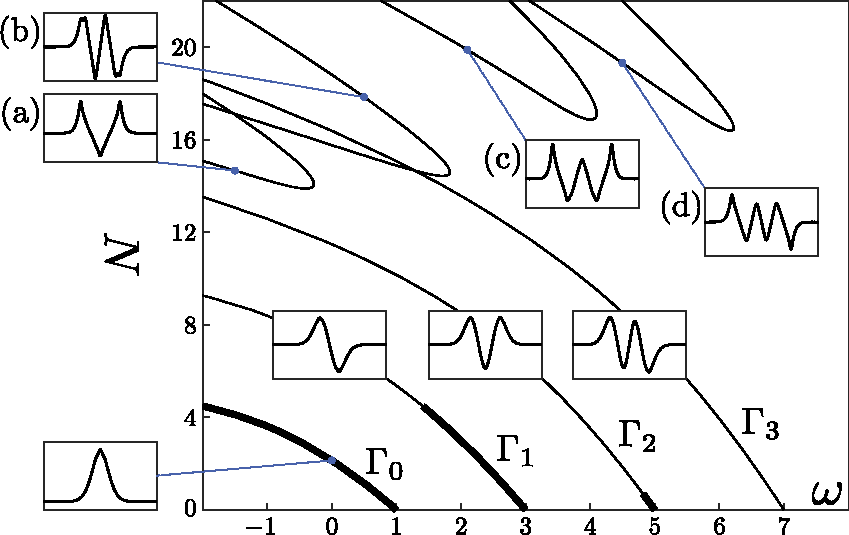
\includegraphics[scale = 1]{pic/branches}
	\caption{
		Диаграммы зависимости нормы решений $N$ от химического потенциала $\omega$, для уравнения \eqref{eq:stationary}; $Q(x) = \omega - x^2$, $P(x) = 1 + 2 \cos (12 x)$.
		Сегменты кривых $N(\omega)$, соответствующие устойчивым решениям, выделены толстыми линями.
		Ветви $\Gamma_n$, $n = 0, 1, 2, 3$ соответствуют семействам решений с линейным аналогом.
	}
\label{fig:branches}
\end{figure}

%\begin{figure}[h]
%\centering
%	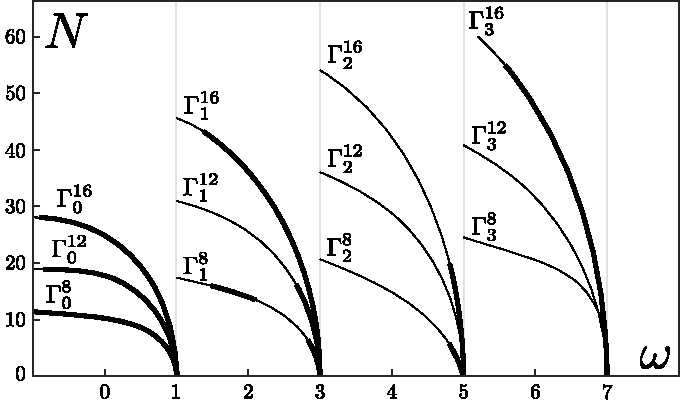
\includegraphics[scale = 1]{pic/branches, different frequencies}
%	\caption{
%		Диаграммы $N(\Omega)$ для ветвей решений с линейным аналогом $\Gamma_n^{\Omega}$, $n = 0, 1, 2, 3$ для уравнения \eqref{eq:stationary}; $Q(x) = \omega - x^2$, $P(x) = \cos \Omega x$, $\Omega = 8, 12, 16$.
%		Сегменты кривых, соответствующие устойчивым решениям, выделены толстыми линями.
%	}
%\label{fig:branches-frequency}
%\end{figure}

В \textbf{заключении (Сonclusion)} подводятся итоги диссертационной работы.
Основные результаты могут быть представлены следующим образом.
\begin{enumerate}
	\item Сформулированы и доказаны общие утверждения о наличии и отсутствии сингулярных решений уравнения \eqref{eq:stationary}.
	\item Сформулированы достаточные условия возможности кодирования регулярных решений уравнения \eqref{eq:stationary} и предложен эффективный алгоритм численной проверки этих условий.
	\item Для случая $U(x) \equiv 0$, $P(x) = A + \cos 2x$ исследовано множество СЛМ уравнения \eqref{eq:gpe} и обнаружено новое устойчивое локализованное решение --- {\it дипольный солитон}.
	\item В случае бесконечной потенциально ямы показано, что присутствие периодического псевдопотенциала приводит к появлению новых классов СЛМ, не имеющих линейных аналогов.
		Для псевдопотенциала с нулевым средним установлено, что увеличение частоты псевдопотенциала приводит к стабилизации малоамплитудных стационарных локализованных решений.
\end{enumerate}

В \textbf{приложении A (Appendix A)} доказывается лемма об ограниченных решениях, использующаяся в первой главе.

В \textbf{приложении B (Appendix B)} в явном виде выписаны решения для двух уравнений типа осциллятора Дуффинга: 
\begin{equation}
	u_{xx} - u + u^3 = 0; \quad u_{xx} - u - u^3 = 0,
\end{equation}
использующиеся в секции 2.3.

В \textbf{приложении C (Appendix C)} приведено доказательство теорем об отображении h- и v-полос, использующихся во второй главе.

% \renewcommand{\bibname}{\protect\leftline{Bibliography}}

\def\thispagestyle#1{}
\renewcommand{\bibname}{\protect\leftline{\large Список публикаций автора по теме диссертации}}
\printbibliography[keyword=own]

% Center aligned bibliography title
% \printbibliography[keyword=own, title={\large Список публикаций автора по теме диссертации}]

% All other cited literature
% \printbibliography[notkeyword=own, title={Цитированная литература}]

\end{document}
